\section{Results}
\label{sec:results}

In this section we demonstrate the utility of our novel framework on three hitherto uninvestigated questions: (i) an exact functional representation of the multi-objective trade-offs in a multi-objective navigation domain; (ii) exact sensitivity analysis of public health policies in epidemic models over the full range of infection rate parameters; and (iii) non-convex optimization of policy parameters applied to finance problems previously impossible with sample-based policy gradient techniques.

\subsection{Multiobjective Navigation}
\label{sec:autonomous_driving}

In this domain we consider an autonomous vehicle moving along one dimension, e.g. along the real number line. At each stage the autonomous vehicle must trade-off between moving into a potentially higher reward region and a cost associated with movement. The domain is specified as follows:
\begin{itemize}
    \item {\footnotesize $ \State = \left\langle loc \right\rangle$}, where $ loc $ is the location of the vehicle
    \item {\footnotesize $ \Action \in \left\lbrace -5.0, 0.0, 5.0 \right\rbrace $} is the amount by which vehicle moves relative to its current location
    \item {\footnotesize 
        \abovedisplayskip=5pt
        \belowdisplayskip=0pt
        \renewcommand{\arraystretch}{1.5}
        \begin{tabular}{ll}
            $ \Transition\left( loc' | loc, a \right) =$ & $ \delta \left[ loc' - (loc + a) \right] $ \\
        \end{tabular}
    }%
    \item {\footnotesize $ \Reward\left(\vec{w}, loc, a, \mathtt{threshold} \right) = w_1 \cdot \Reward_{\mathtt{location}} + w_2 \cdot \Reward_{\mathtt{movement}} $} where, \\
    {\footnotesize 
        \abovedisplayskip=10pt
        \belowdisplayskip=0pt
        \renewcommand{\arraystretch}{1.5}
        \begin{tabular}{ll}    
            $ \Reward_{\mathtt{location}}(loc', a, \mathtt{threshold}) = $ &  $ $ \\
                \qquad $ \begin{cases}
                (loc' \geq \mathtt{threshold}) : & loc' \\
                \text{otherwise} : & 0.0 \\
                \end{cases} $ & $ $\\
            $ \Reward_{\mathtt{movement}}(loc', a) = -cost_{\mathtt{movement}} $ & $ $ \\                        
        \end{tabular}
    }    
\end{itemize} 

In Figure~\ref{fig:vehicle1d} we present the optimal $ \Horizon = 10 $ value function for the multiobjective navigation domain with $ \mathtt{threshold} = 10.0 $ and $ cost_{\mathtt{movement}} = -1.0 $.

%------------------------------------------------------------------------------
% Figure
\begin{figure}[h!]
    \centering
    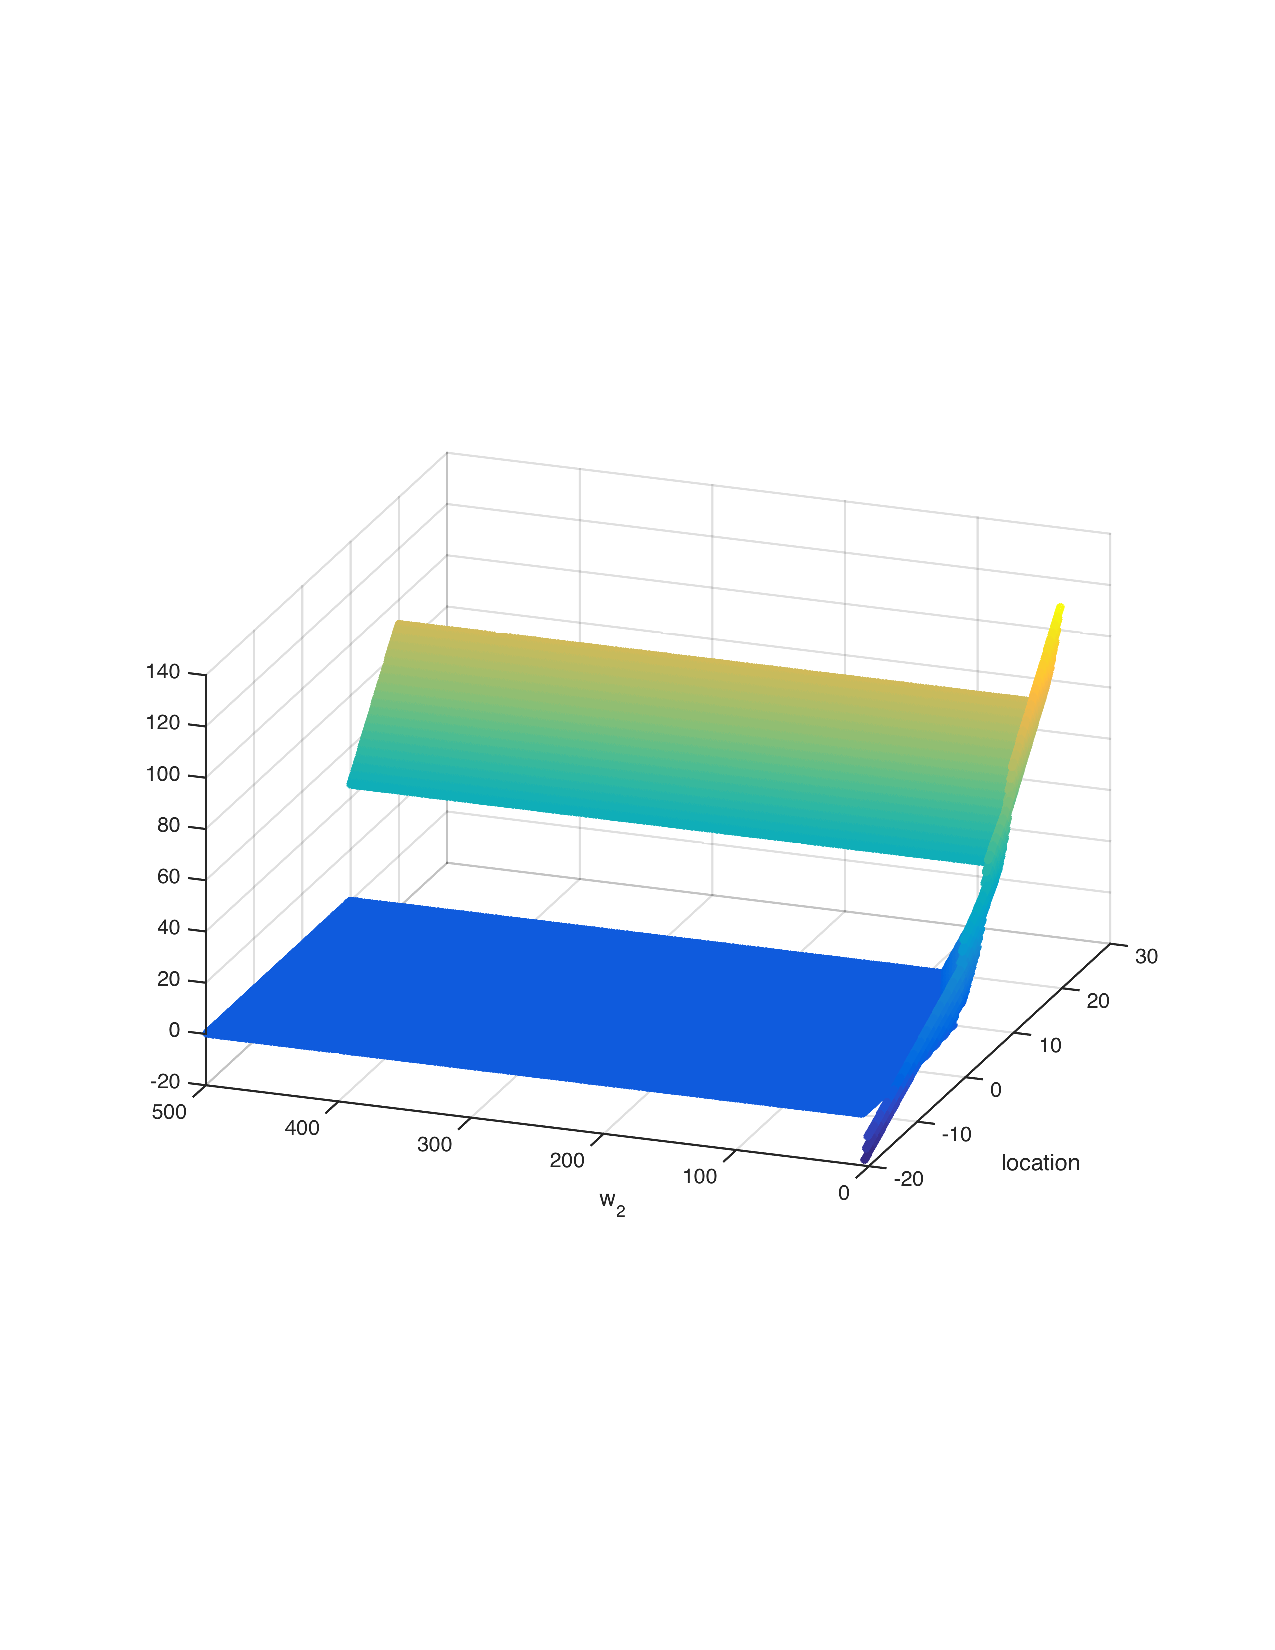
\includegraphics[width=\linewidth, height=0.8\linewidth]{images/robot1d}
    \caption{The optimal $ \Horizon = 10 $ value function for the multiobjective navigation domain. }
    \label{fig:vehicle1d}
\end{figure}
%------------------------------------------------------------------------------

\subsection{Influenza Public Health Policy}
\label{sec:results_influenza}

Influenza viruses continuously challenge both human and avian posts with new variants causing complex epidemics. Compartmental models are widely used within epidemiology to investigate the spread of infection diseases. In this domain we investigate the sensitivity of two different Influenza models to an infection rate parameter. 

\subsubsection{S-D Model}

The first model is defined as follows:
\begin{align*}
    s_{t + 1} &= - s_t \cdot ( \eta + a ) \\
    d_{t+1} &= \eta \cdot s_t 
\end{align*}
where {\footnotesize $ \eta \in [0, 1]$} is the rate of infection and {\footnotesize $ a_t \in \left\lbrace 0, \ldots, 1.0\right\rbrace $} is the proportion of susceptibles {\footnotesize $ s_t $} to be vaccinated. The model can be formulated as follows:
\begin{itemize}
    \item {\footnotesize $ \State = \left\langle S, D \right\rangle$ }, where $ s $ and $ d $ are as defined above
    \item {\footnotesize $ \Action \in \left\lbrace 0, 0.25, 0.50, 1.0 \right\rbrace $} is the proportion of $ S $ to vaccinate
    \item The transition function {\footnotesize \Transition} for each state variable in {\footnotesize \State} is given by:    \\
    {\footnotesize 
        \abovedisplayskip=5pt
        \belowdisplayskip=0pt
        \renewcommand{\arraystretch}{1.5}
        \begin{tabular}{ll}
            $ \Transition\left( s' | s, d, a \right) =$ & $ \delta \left[ s' - (- s \cdot (\eta + a)) \right] $ \\
            $ \Transition\left( d' | s, d, a \right) =$ & $ \delta \left[ d' - (\eta \cdot s) \right] $ \\
        \end{tabular}
    }%
    \item {\footnotesize $ \Reward\left(\vec{w}, cost_{\mathtt{death}}, cost_{\mathtt{vaccine}}, s, d, a \right) = w_1 \cdot \Reward_{\mathtt{death}} + w_2 \cdot \Reward_{\mathtt{vaccine}}$} where, {\footnotesize $ cost_{\mathtt{inf}} $} is the incident cost of infection and {\footnotesize $ cost_{\mathtt{vaccine}} $} is the unit cost of vaccination \\
    {\footnotesize 
        \abovedisplayskip=10pt
        \belowdisplayskip=0pt
        \renewcommand{\arraystretch}{1.5}
        \begin{tabular}{ll}    
            $ \Reward_{\mathtt{death}}(s', d', a, cost_{\mathtt{death}}) = $ &  $ $ \\
                \qquad $ \begin{cases}
                (d \geq 0) : & cost_{\mathtt{death}} \cdot d \\
                \text{otherwise} : & 0 \\
                \end{cases} $ & $ $ \\
            $ \Reward_{\mathtt{vaccine}}(s', d', a, cost_{\mathtt{vaccine}}) = $ &  $ $ \\
                \qquad $ \begin{cases}
                (s \geq 0) : & cost_{\mathtt{vaccine}} \cdot s \cdot a \\
                \text{otherwise} : & 0 \\
                \end{cases} $ & $ $ \\
        \end{tabular}
    }    
\end{itemize} 

Figure~\ref{fig:influenza_sd} shows the optimal {\footnotesize$ \Horizon = 4 $} value function for the SD formulation of the influenza domain. The parameters of the models were set to $cost_{\mathtt{inf}} = 95.0$ and $cost_{\mathtt{vaccine}} = 33.0$.

%------------------------------------------------------------------------------
% Figure
\begin{figure}[h!]
    \centering
    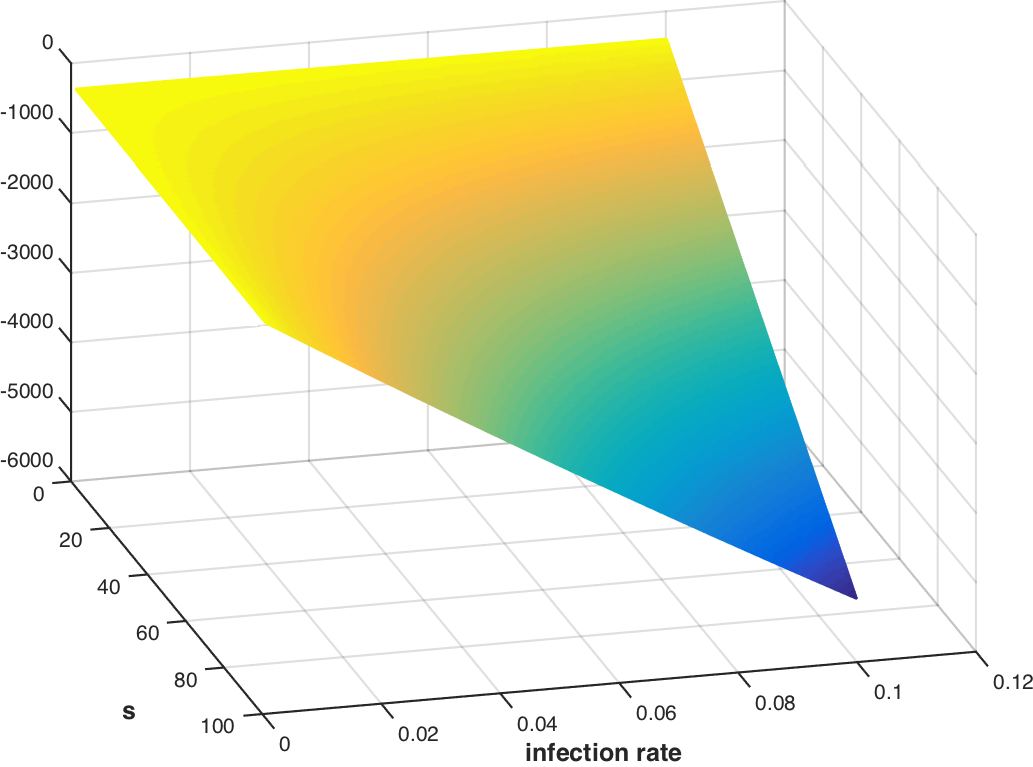
\includegraphics[width=\linewidth, height=0.8\linewidth]{images/sd_infection_s}
    \caption{Optimal $ \Horizon = 4 $ Influenza Epidemiology value under the S-D and S-D specification.}
    \label{fig:influenza_sd}
\end{figure}
%------------------------------------------------------------------------------

\subsubsection{S-I-R-S Model}

An alternate Influenza can be defined as follows:
\begin{align*}
    s_{t + 1} &= -\eta \cdot s_t \cdot i_t + c \cdot r_t - a_t \cdot s_t \\
    i_{t + 1} &= \eta \cdot s_t \cdot i_t - b \cdot i_t \\
    r_{t+1} &= b \cdot i_t - c \cdot r_t 
    %    d_{t+1} &= e \cdot i_t 
\end{align*}

The Influenza SIR model can be formulated as an parameterized MDP as follows:
\begin{itemize}
    \item {\footnotesize $ \State = \left\langle S, I, R \right\rangle$ }, where $ S $, $ I $, and $ R $ are as defined above
    \item {\footnotesize $ \Action \in \left\lbrace 0, 0.25, 0.50, 1.0 \right\rbrace $} is the proportion of $ S $ to vaccinate
%\end{itemize}
%\begin{itemize}
    \item The transition function {\footnotesize \Transition} for each state variable in {\footnotesize \State} is given by:    
    {\footnotesize 
        \abovedisplayskip=5pt
        \belowdisplayskip=0pt
        \renewcommand{\arraystretch}{1.5}
        \begin{tabular}{ll}
            $ \Transition\left( s' | s, i, r, a \right) =$ & $ \delta \left[ s' - (- \eta \cdot s \cdot i + c \cdot r -a \cdot s) \right] $ \\
            $ \Transition\left( i' | s, i, r, a \right) =$ & $ \delta \left[ i' - (\eta \cdot s \cdot i - b \cdot i) \right] $ \\
            $ \Transition\left( r' | s, i, r, a \right) =$ & $ \delta \left[ r' - (b \cdot i - c \cdot r) \right] $ \\            
        \end{tabular}
    }%
    \item {\footnotesize $ \Reward\left(\vec{w}, cost_{\mathtt{inf}}, s, i, r, a \right) = w_1 \cdot -cost_{\mathtt{inf}} \cdot i + w_2 \cdot -cost_{\mathtt{vaccine}} \cdot a $}, where {\footnotesize $ cost_{\mathtt{inf}} $} is the incident cost of infection and {\footnotesize $ cost_{\mathtt{vaccine}} $} is the unit cost of vaccination \\
\end{itemize} 

Figure~\ref{fig:influenza_sirs} shows the optimal {\footnotesize$ \Horizon = 4 $} value function for the S-I-R-S formulation of the influenza domain. The parameters of the models were set to $b = 0.27, c = 0.23, cost_{\mathtt{inf}} = 95.0$ and $cost_{\mathtt{vaccine}} = 33.0$.

%------------------------------------------------------------------------------
% Figure
\begin{figure}[t!]
    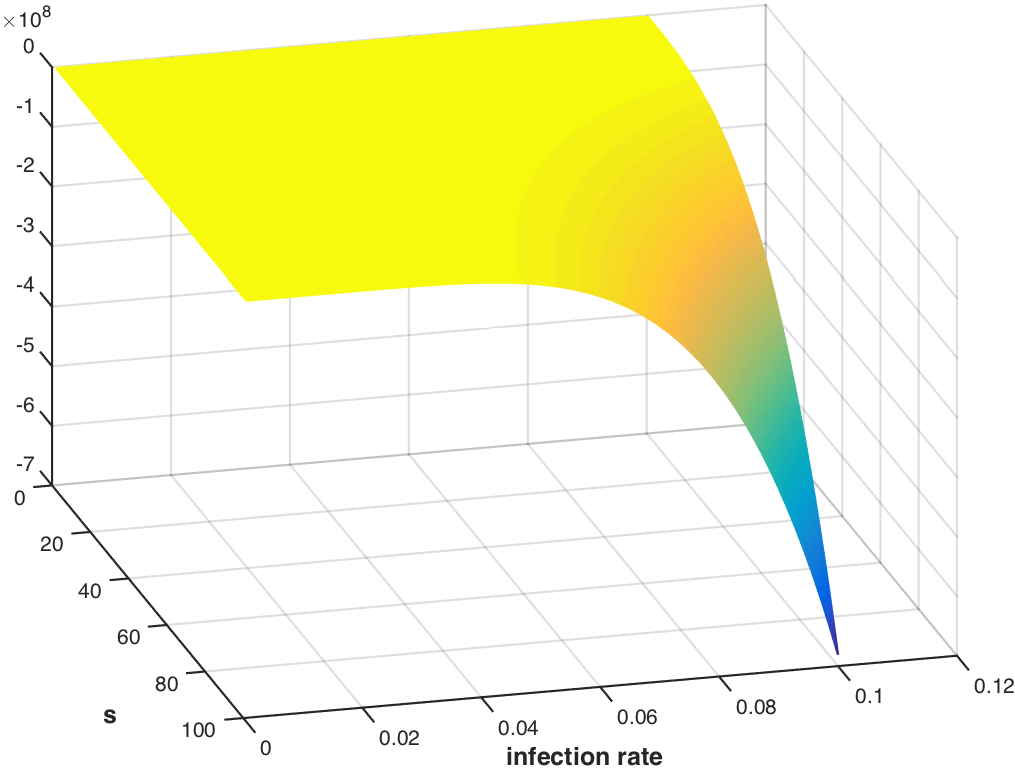
\includegraphics[width=\linewidth, height=0.8\linewidth]{images/sir_infection_s}
    \caption{Optimal $ \Horizon = 4 $ Influenza Epidemiology value under the S-D and S-I-R-S specification.}
    \label{fig:influenza_sirs}
\end{figure}
%------------------------------------------------------------------------------

%\subsection{Influenza Epidemiology Susceptible-Infected-Recovered-Susceptible}
%\label{sec:results_ee}
%
%We can describe Influenza epidemics by an SIRS (Susceptible-Infective-Recovered-Susceptible) model. {\footnotesize $ S $} refer to the number of susceptibles, {\footnotesize $ I $} to number of infected and {\footnotesize $ R $} to the recovered. At each time step the population in each of the three populations is updated according to the following equations:
%\begin{align*}
%    s_{t + 1} &= -\eta \cdot s_t \cdot i_t + c \cdot r_t - a_t \cdot s_t \\
%    i_{t + 1} &= \eta \cdot s_t \cdot i_t - b \cdot i_t \\
%    r_{t+1} &= b \cdot i_t - c \cdot r_t 
%%    d_{t+1} &= e \cdot i_t 
%\end{align*}
%
%where {\footnotesize $ \eta \in [0, 1]$} is the rate of infection, {\footnotesize $ b \in [0, 1]$} is the rate of recovery and {\footnotesize $ c \in [0, 1]$} is the rate of susceptibility. At each decision epoch we allow a proportion of susceptibles {\footnotesize $ s_t $} to be immunised i.e. {\footnotesize $ a_t \in \left\lbrace 0, \ldots, 1.0\right\rbrace $}. The Influenza SIR model can be formulated as an MOMDP as follows:
%
%\begin{itemize}
%    \item {\footnotesize $ \State = \left\langle S, I, R \right\rangle$ }, where $ S $, $ I $, and $ R $ are as defined above
%    \item {\footnotesize $ \Action \in \left\lbrace 0, 0.25, 0.50, 1.0 \right\rbrace $} is the proportion of $ S $ to vaccinate
%%\end{itemize}
%%\begin{itemize}
%    \item The transition function {\footnotesize \Transition} for each state variable in {\footnotesize \State} is given by:    
%    {\footnotesize 
%        \abovedisplayskip=5pt
%        \belowdisplayskip=0pt
%        \renewcommand{\arraystretch}{1.5}
%        \begin{tabular}{ll}
%            $ \Transition\left( s' | s, i, r, a \right) =$ & $ \delta \left[ s' - (- \eta \cdot s \cdot i + c \cdot r -a \cdot s) \right] $ \\
%            $ \Transition\left( i' | s, i, r, a \right) =$ & $ \delta \left[ i' - (\eta \cdot s \cdot i - b \cdot i) \right] $ \\
%            $ \Transition\left( r' | s, i, r, a \right) =$ & $ \delta \left[ r' - (b \cdot i - c \cdot r) \right] $ \\            
%        \end{tabular}
%    }%
%    \item {\footnotesize $ \Reward\left(\vec{w}, cost_{\mathtt{inf}}, s, i, r, a \right) = w_1 \cdot -cost_{\mathtt{inf}} \cdot i + w_2 \cdot -cost_{\mathtt{vaccine}} \cdot a $}, where {\footnotesize $ cost_{\mathtt{inf}} $} is the incident cost of infection and {\footnotesize $ cost_{\mathtt{vaccine}} $} is the unit cost of vaccination \\
%\end{itemize} 

%%------------------------------------------------------------------------------
%% Figure
%\begin{figure}[t!]
%    \centering
%    \begin{subfigure}[b]{0.4\textwidth}
%        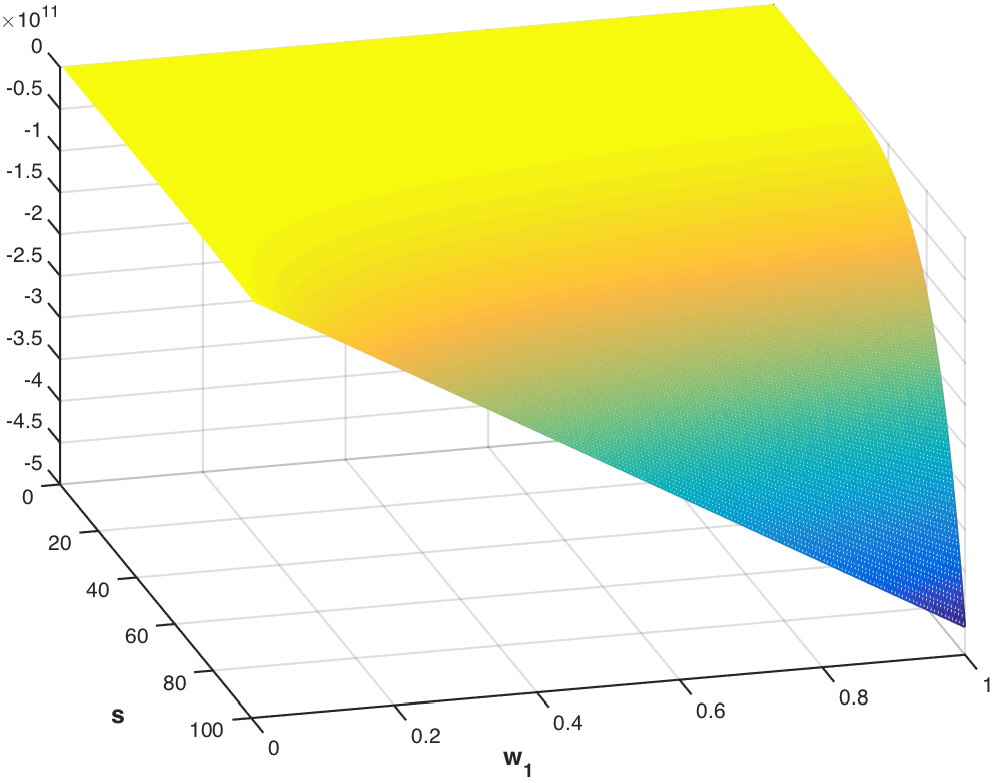
\includegraphics[width=\linewidth, height=0.8\linewidth]{images/sir_s_w1}
%        \caption{$ s \in \left[ 0.0, 100.0 \right], w_1 \in \left[ 0.0, 100.0 \right], i = 50.0, r = 50.0$}
%        \label{fig:sir_s_w1}
%        \vspace{1em}
%    \end{subfigure}
%    
%    \begin{subfigure}[b]{0.4\textwidth}
%        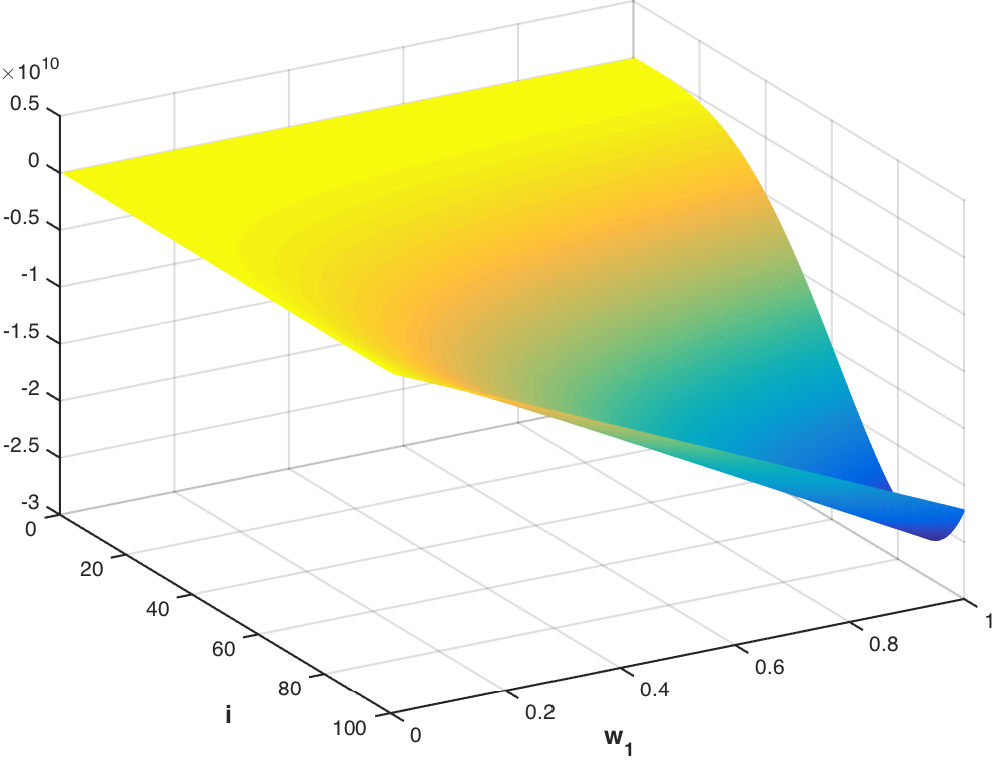
\includegraphics[width=\linewidth, height=0.8\linewidth]{images/sir_i_w1}
%        \caption{$ i \in \left[ 0.0, 100.0 \right],w_1 \in \left[ 0.0, 100.0 \right], s = 50.0, r = 50.0$}
%        \label{fig:sir_i_w1}
%    \end{subfigure}  
%    
%    \begin{subfigure}[b]{0.4\textwidth}
%        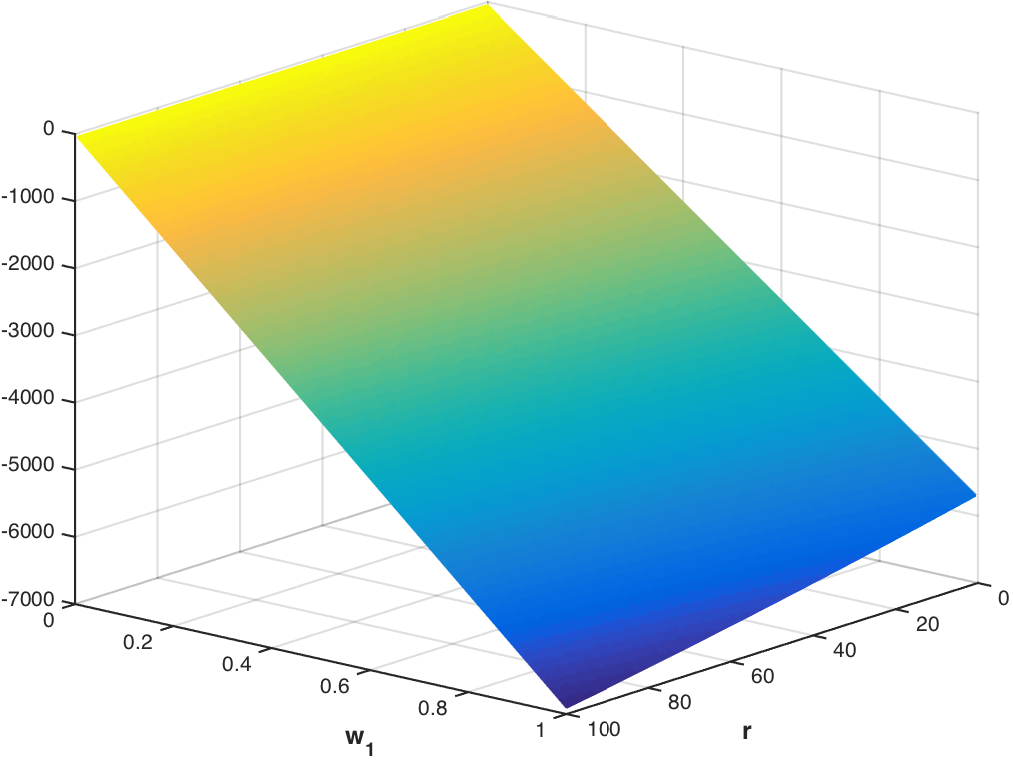
\includegraphics[width=\linewidth, height=0.8\linewidth]{images/sir_r_w1}
%        \caption{$ r \in \left[ 0.0, 100.0 \right], w_1 \in \left[ 0.0, 100.0 \right], s = 50.0, i = 50.0$}
%        \label{fig:sir_r_w1}
%    \end{subfigure}      
%    \caption{Influenza S-I-R-S Epidemiology. $ \Horizon = 15 $, $ \eta = 1.65 \times 10^2, b = 0.27, c = 0.23, cost_{\mathtt{inf}} = 95.0, cost_{\mathtt{vaccine}} = 33.0$.}
%    \label{fig:sir}
%\end{figure}
%%------------------------------------------------------------------------------

\subsection{Optimal Execution}
\label{sec:results_oe}

Institutional investors often need to acquire or liquidate a number of shares within a given period of time. Indirect transaction costs are an important consideration for institutional investors who often want to transact a number of shares that exceeds the available liquidity i.e. there may not be counterparty or counterparties that wish to take the other side of the trade at the same volume. There is a clear trade-off between the market impact of transacting immediately and the volatility of slow execution. 

In this domain we investigate the optimal execution problem using a price impact model inspired by Bertsimas and Lo~\parencite{Bertsimas_JFM_1998} as follows:
\begin{itemize}
    \item {\footnotesize $ \State = \left\langle price, inv \right\rangle$}, where $ price $ is the price of the asset and $ inv $ is the inventory remaining 
    \item {\footnotesize $ \Action \in \left\lbrace 0, 0.25, 0.50, 1.0 \right\rbrace $} is the proportion of the remaining inventory sell
    \item The transition function {\footnotesize \Transition} for each state variable in {\footnotesize \State} is given by:    \\
    {\footnotesize 
        \abovedisplayskip=5pt
        \belowdisplayskip=0pt
        \renewcommand{\arraystretch}{1.5}
        \begin{tabular}{ll}
            $ \Transition\left( price' | price, inv, n \right) = $ & $ $ \\
                $ \qquad \delta \left[ price' - \begin{cases}
                n \geq 0  : & price + \theta \cdot n + \sigma \cdot \epsilon_{t+1} \\
                \text{otherwise} : & price + \sigma \cdot \epsilon_{t+1} \\
                \end{cases} \right] $ & $ $\\            
            $ \Transition\left( inv' | price, inv, n \right) = $ & $ $ \\
                $ \qquad \delta \left[ i' - \begin{cases}
                n \geq 0 : & inv - inv \cdot n \\
                \text{otherwise} : & i \\
                \end{cases} \right] $ & $ $\\
        \end{tabular}
    }%
    \item {\footnotesize $ \Reward\left(\vec{w}, price, price_0, inv, n \right) = w_1 \cdot \Reward_{\mathtt{inventory}} - w_2 \cdot \Reward_{\mathtt{shortfall}} $} where, \\
    {\footnotesize 
        \abovedisplayskip=10pt
        \belowdisplayskip=0pt
        \renewcommand{\arraystretch}{1.5}
        \begin{tabular}{ll}    
            $ \Reward_{\mathtt{inventory}}(price', inv', n) = $ &  $ $ \\
                \qquad $ \begin{cases}
                (inv \geq 0) : & -inv \\
                \text{otherwise} : & 0 \\
                \end{cases} $ & $ $ \\           
            $ \Reward_{\mathtt{shortfall}}(price', price_0, inv', n) = $ &  $ $ \\
                \qquad $ \begin{cases}
                (n \geq 0) : & n \cdot inv \cdot price - inv \cdot price_0 \\
                \text{otherwise} : & 0 \\
                \end{cases} $ & $ $ \\           
        \end{tabular}
    }    
\end{itemize}

The investor aims to liquidate inventory via {\footnotesize $ \Reward_{\mathtt{inventory}} $} and minimise implementation shortfall via {\footnotesize $ \Reward_{\mathtt{shortfall}} $}. Implementation shortfall is defined as the difference
between the theoretical benchmark price and the actual price received is the implementation shortfall~\parencite{Perold_JPM_1988}.

%------------------------------------------------------------------------------
% Figure
\begin{figure}[t!]
    \centering
    \begin{subfigure}[b]{0.4\textwidth}    
%        \centering
        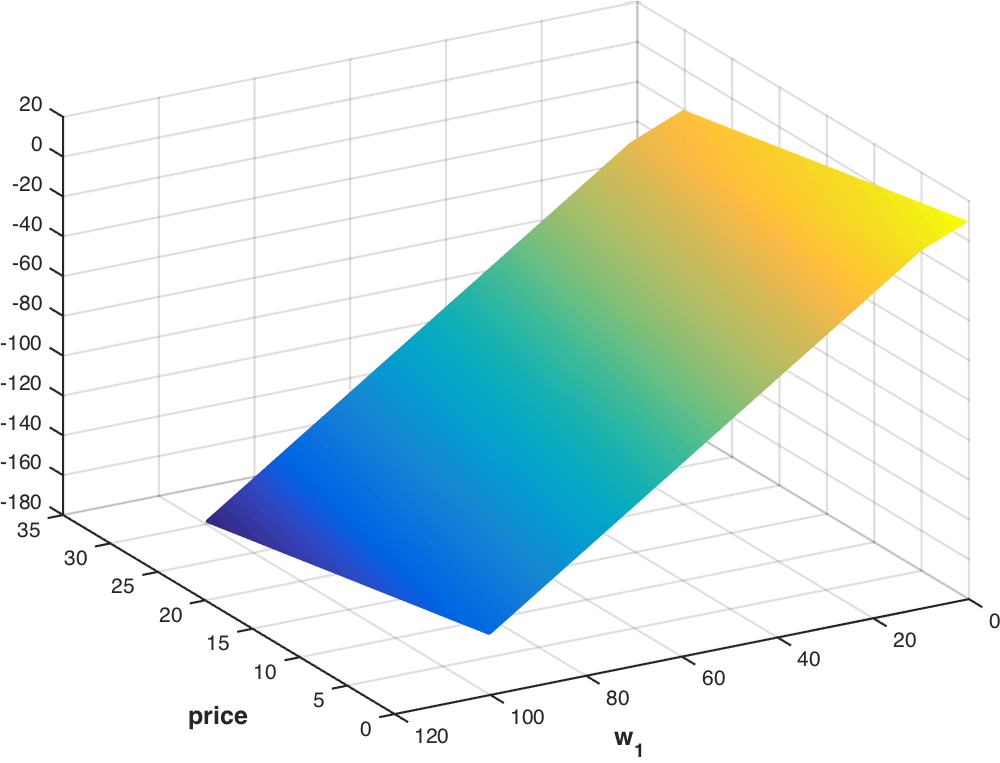
\includegraphics[width=\linewidth, height=0.8\linewidth]{images/opt_execution_w1}
        \caption{$ w_1 \in \left[ 0.0, 100.0 \right]$}
        \label{fig:opt_execution_w1}
        \vspace{1em}
    \end{subfigure}
    
    \begin{subfigure}[b]{0.4\textwidth}    
%        \centering
        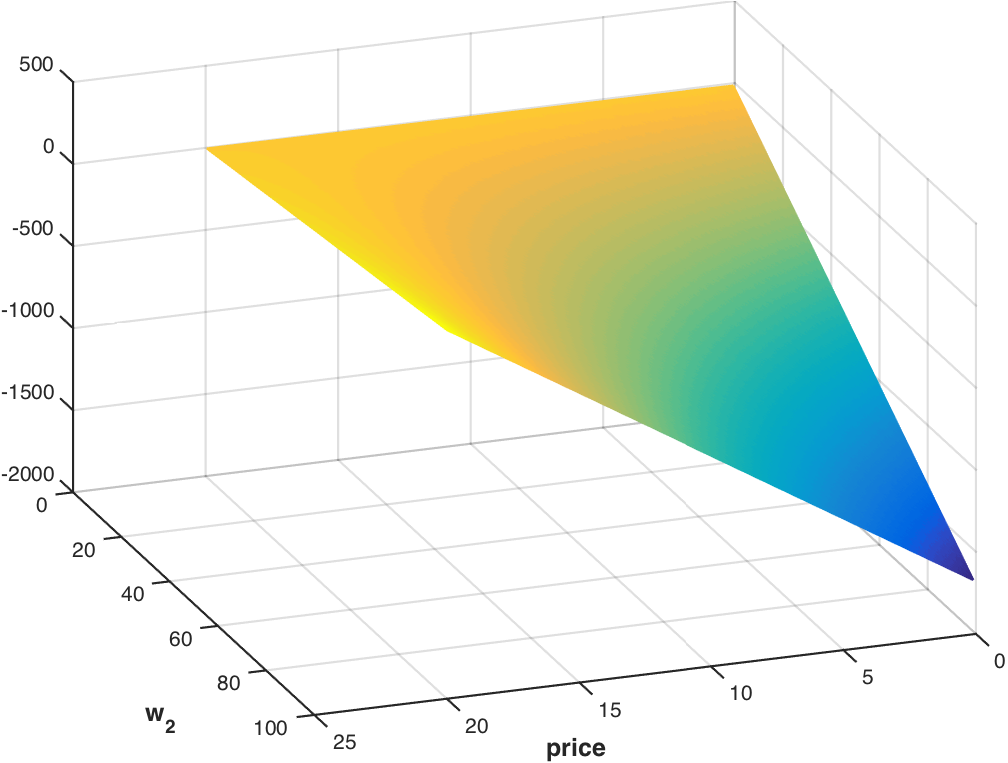
\includegraphics[width=\linewidth, height=0.8\linewidth]{images/opt_execution_w2}
        \caption{$ w_2 \in \left[ 0.0, 100.0 \right]$}
        \label{fig:pt_execution_w2}
    \end{subfigure}  
    \caption{Optimal Execution. $ \Horizon = 5 $, $ price \in \left[ 0.0, 20.0 \right]$, $ price_0 = 10.0, i = 1.0$.}
    \label{fig:pt_execution}
\end{figure}
%------------------------------------------------------------------------------